\begin{figure}[htbp]
\centering
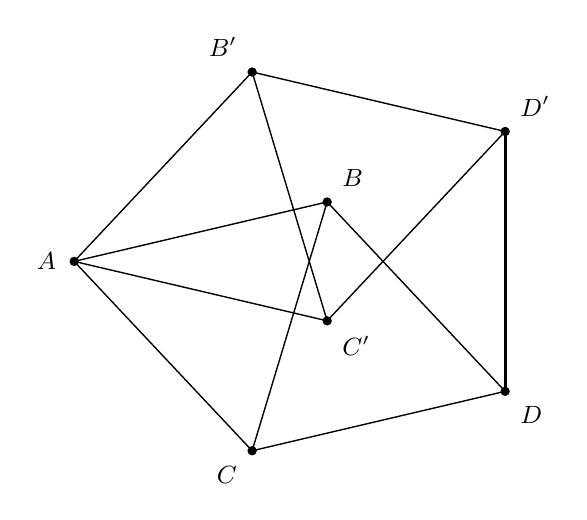
\begin{tikzpicture}[scale=3.3, every node/.style={font=\small}]
  % The long diagonals AD and AD' have length sqrt(3). Their angles are
  % -alpha and +alpha, where alpha = asin(1/(2 sqrt(3))).
  \coordinate (A)  at (0,0);
  \coordinate (B)  at (0.973493765,0.228713554);
  \coordinate (C)  at (0.684818630,-0.728713554);
  \coordinate (D)  at (1.658312395,-0.500000000);
  \coordinate (Bp) at (0.684818630,0.728713554);
  \coordinate (Cp) at (0.973493765,-0.228713554);
  \coordinate (Dp) at (1.658312395,0.500000000);
  \draw[line width=0.5pt] (A)--(B)--(D)--(C)--cycle;
  \draw[line width=0.5pt] (B)--(C);
  \draw[line width=0.5pt] (A)--(Bp)--(Dp)--(Cp)--cycle;
  \draw[line width=0.5pt] (Bp)--(Cp);
  \draw[line width=1pt] (D)--(Dp);
  \fill (A) circle (0.018) node[left=3pt] {$A$};
  \fill (B) circle (0.018) node[above right=2pt] {$B$};
  \fill (C) circle (0.018) node[below left=2pt] {$C$};
  \fill (D) circle (0.018) node[below right=2pt] {$D$};
  \fill (Bp) circle (0.018) node[above left=2pt] {$B'$};
  \fill (Cp) circle (0.018) node[below right=2pt] {$C'$};
  \fill (Dp) circle (0.018) node[above right=2pt] {$D'$};
\end{tikzpicture}
\caption{Two unit rhombi sharing $A$, with the second rotated by $\theta$ where $2\sqrt3\sin(\theta/2)=1$. The heavier edge joins $D$ and $D'$; all eleven drawn edges have unit length.}
\label{fig:moser}
\end{figure}
